\chapter{The IMF Eco-System }
\label{ch:Chapter 7}
IMF will be implemented in the context of applications that serve
different parts of an eco-system. The applications in the IMF Eco-System should enable the engineers to create and
share Information Models with minimal training and independent of companies and industries. An overview of the
different components in the eco-system are shown in \autoref{fig:Figure 54}. The main components are RDL, IMF Type Library,
Authoring Tools, and Data Exchange Formats. In this chapter all references to applications in the IMF eco-system are
made to the type of application, not to a specific instance of the applications unless otherwise stated.


\begin{figure}[htb]
  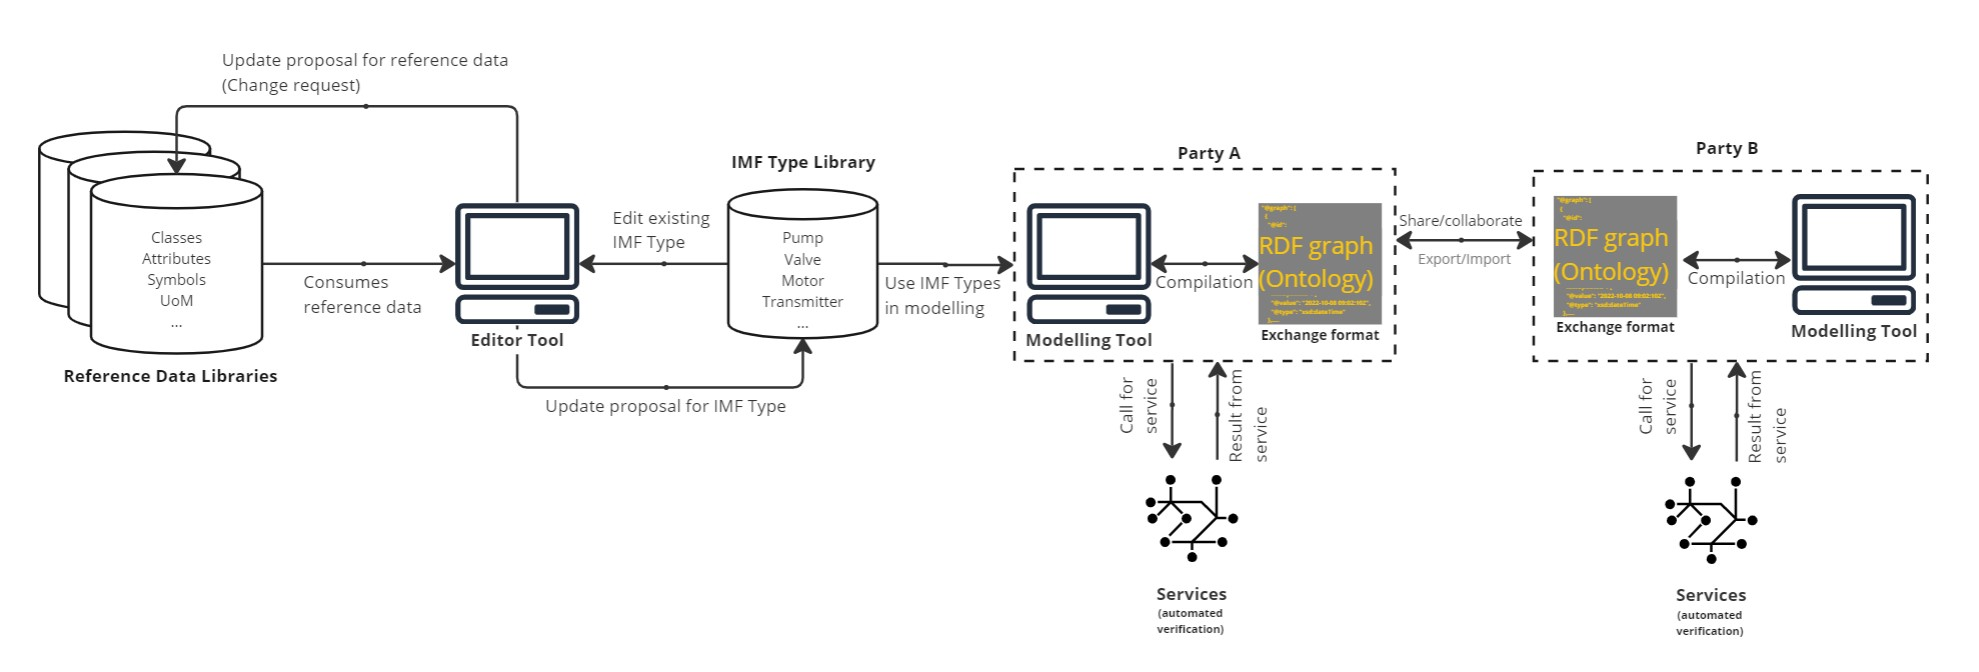
\includegraphics[width=1\textwidth]{img/IMFmanual-img072.jpg}
  \caption{Overview of the IMF Eco-System.}
  \label{fig:Figure 54}
\end{figure}

\section{Reference Data Library and IMF Type Library}
\subsection{Reference Data Library}
RDLs are industry shared resources and thus enable standardization as well as minimizing
duplication of work. IMF can make use of different RDLs and align them as part of the IMF Model integration process.
IMF Models draw on a shared resource of definitions such as IMF Types and classes, property vocabularies, and units
of measure. For example, when referring to an IMF Type in the IMF Model, the IMF Type must be from a list of allowed
types, and the IMF Type itself must be defined. For this the shared resource is the master, and the reference data is
available, for instance in a look-up fashion, when building the IMF Model.

The commercial benefits of deploying the IMF across industry, enabling shared resources and re-use are strong, but in
some cases competitive advantage takes priority, with the need to protect Intellectual Property (IP). The IMF fully
accommodates this need. Reference data, design codes, and model blocks can be proprietary, in which case they could
be hosted by the owner, instead of hosted by an industry service (such as PCA).

\subsection{IMF Type Library}
IMF Type Library is a common industry resource for sharing IMF Types between IMF users. A
common industry library of IMF Types will increase the standardization of IMF Types, reduce duplicate work, and make
adaptation of IMF easier for new users.

The IMF Type Library shall offer support for:

\begin{itemize}
  \item Submitting suggestions for new and updating existing IMF Types.
  \item Quality Assurance process for approval of suggestions for new and updating existing IMF Types. The QA workflow
        shall be transparent and offer relevant tools for an efficient and easy to use workflow.
  \item Versioning scheme for the entries in the library.
  \item API that allows for querying the library.
  \item Classification schema for the IMF Types.
\end{itemize}
IMF Type Library shall be community driven by allowing all IMF users to submit new IMF types and updating already
existing IMF types in the library. This will allow users across the industry and value chain to collaborate to create
high quality content. The approval process can be implemented as a peer-review where groups of SMEs can collaborate
to ensure that updates to the library have the necessary quality.

The IMF Type Library is used to store and distribute the IMF Types created using the IMF Type Tool and as a source for
IMF Types for the modelling. The API of the IMF Type Library shall offer support for the necessary functionality in
the IMF Type Tool and the IMF Modelling Tool.

\section{Authoring Tools}
The Authoring Tools are the front-end tools used by the SMEs to create IMF Types and IMF
Models. These tools can be implemented as standalone products or be integrated into already existing engineering
tools. To offer seamless integration with the other components in the IMF eco-system the implementation of the
authoring tools shall comply with the requirements outlined in the IT-specification that will be issued at a later
stage.

\subsection{IMF Type Editor Tool}
The IMF Type Editor Tool is used to create new IMF Types and populate the IMF Type library
that is used in the modelling.

The IMF Type Editor Tool shall offer support for:

\begin{itemize}
  \item Search and browse for existing IMF Types in the IMF Type Library.
  \item Source attributes, classes, etc. from the Reference Data Library.
  \item Creation of new IMF Types (aspect blocks, terminals, interface points) using a graphical user interface.
  \item Updating existing IMF Types in the IMF Type Library.
  \item Workflow for submitting new or updating existing IMF Types in the IMF Type Library.
  \item Workflow for submitting suggestions for new reference data entries to the Reference Data Library.
\end{itemize}
To increase the standardization of the types created using an IMF Type Editor Tool, the Reference Data Library
previously described shall be used for sourcing attributes, symbols, and classes for the creation of IMF Types. There
should be a workflow that allows the SME to submit suggestions for new reference data entries to the RDL that are
identified as missing during the IMF Type creation process.

\subsubsection{Open-Source tool \emph{:Tyle}}

The IMF Type Editor Tool \emph{:Tyle }has been developed to offer adopters of IMF a web-based open-source IMF Type
Editor. \emph{:Tyle }supports creation of aspect blocks, interface points and terminals using the POSC Caesar
Association RDL and IMF Type Library. \emph{:Tyle} is developed as an open source project, where all users are
invited to contribute to the development of the tool by submitting code, bug reports or feature requests. Source
code, documentation and user tutorials can be found on
\href{https://github.com/mimir-org/typelibrary}{Github}.

\subsection{IMF Modelling Tool}
The IMF Modelling Tool is used by the SME to create the IMF Models and translate the
created models into ontologies that can be shared across the value chain.

The IMF Modelling Tools shall offer support for:

\begin{itemize}
  \item Searching and browsing for types in the IMF Type Library.
  \item Creation of models using a graphic interface (block diagram) that allows instantiation of aspect blocks, and
        configuration of all topological and hierarchical relations between aspect blocks, including inter-aspect relations.
  \item Modelling in all aspects in the core IMF (function, product, location, installed).
  \item Translate the models into ontologies according to the IMF specification.
  \item Export/Import IMF Models to/from the standardized IMF Model exchange format.
  \item Plugins that can perform specific calculations and queries.
\end{itemize}
IMF Modelling Tools shall source the IMF Types from the IMF Type Library. The sourced IMF Types are then instantiated
in the modelling tool. Setting the values or references to values for the different attributes of the IMF Types shall
be possible in the modelling tool.

The IMF Modelling Tool should provide a framework for adding plugins that can perform calculations and queries on a
model. Use cases include checking that products that are related to functions fulfil the requirements stated by the
function.


\subsubsection{Open-Source Tool \emph{Mímir}}

The open-source IMF Modeling Tool \emph{Mímir} has been developed to offer adopters of IMF a web-based open-source
modelling tool. It supports creation of models, sourcing types from an IMF Type Library and compiling the models into
ontologies. All users are welcome to contribute to the development of \emph{Mímir} by submitting code, bug reports
or feature requests. Source code, documentation and tutorials can be found on
\href{https://github.com/mimir-org/mimir}{Github}.

\section{Serialization and Data Exchange}
The IMF Eco-System is intended to be an industry wide collaboration that allows transfer
of Information Models between the different parts of the value chain (operators, engineering contractors, suppliers).
To enable seamless transfer of Information Models between the different actors, potentially using different
applications, a standardized serialization and data exchange format is needed.

The data exchange format will be defined using widely accepted W3C standards. The IMF data exchange format is Resource
Description Framework (RDF), using any of its widely supported standardized serialization formats. Several
serialization formats for RDF exist, including JSON-LD, which is based on JSON, and RDF/XML, which is based on XML.
The data exchange format vocabulary will be specified using the Web Ontology Language (OWL) and its grammar will be
defined by the Shapes Constraint Language (SHACL). The vocabulary and grammar specification of the data exchange
format will encompass the semantics and constraints of the vocabulary and grammar specifications of the formal IMF
language to the degree that OWL and SHACL languages support this and in a way that semantic and syntactic
verification of the exchanged data may be practically applied.
